%%%%%%%%%%%%%%%%%%%%%%%%%%%%%%%%%%% Einstellungen/Vorgaben %%%%%%%%%%%%%%%%%%%%%%%%%%%%%%%%%%%

% Basics
\documentclass[ngerman, a4paper, 12pt, oneside, pdftex]{report}

% UTF-8 codierung verwenden
\usepackage[utf8]{inputenc}

\clubpenalty = 10000
\widowpenalty = 10000
\displaywidowpenalty = 10000

% Nützliche Packages
\usepackage[T1]{fontenc}
\usepackage{lmodern} % Vektor-Schriftart
\usepackage{geometry} % Seitenränder
\usepackage{graphicx} % Grafiken
\usepackage{caption} % Bildunterschriften etc.
\usepackage{acronym} % Abkürzungen
\usepackage{listings} % Listenverzeichnis
\usepackage{color} % Benutzerdefinierte Farben
\usepackage{csquotes}
\usepackage{svg} % Vektor-Grafiken
\usepackage{enumitem}
\usepackage{tcolorbox}
\usepackage[htt]{hyphenat}
\usepackage{scrextend}
\usepackage[bottom]{footmisc}
\usepackage[german]{babel}
%\usepackage[backend=biber,maxcitenames=3,hyperref=true,bibencoding=inputenc,style=alphabetic,citestyle=alphabetic]{biblatex} % Literaturverzeichnis
\usepackage{setspace}
%\usepackage[nottoc, notlof, notlot]{tocbibind}
\usepackage[headsepline]{scrpage2} % Kopf- und Fusszeilen

% Farben
\definecolor{dkgreen}{rgb}{0,0.6,0}
\definecolor{gray}{rgb}{0.5,0.5,0.5}
\definecolor{mauve}{rgb}{0.58,0,0.82}

% Code-Embedding
\lstset{frame=single,
  language=Java,
  aboveskip=3mm,
  belowskip=3mm,
  showstringspaces=false,
  columns=flexible,
  basicstyle={\small\ttfamily},
  numbers=left,
  numberstyle=\tiny\color{gray},
  keywordstyle=\color{blue},
  commentstyle=\color{dkgreen},
  stringstyle=\color{mauve},
  keepspaces=true,
  breaklines=true,
  breakatwhitespace=true,
  tabsize=3
}

% Sprache
\selectlanguage{german}

% Seitenränder
\geometry{left=25mm, right=25mm, top=25mm, bottom=25mm} % bindingoffset=5mm

\setlength{\headheight}{1.1\baselineskip}

% Zeilenabstand 1.5
\onehalfspacing

% Caption Setup
\captionsetup{labelfont=bf, textfont=normalfont}

% Verfasser
\newcommand{\Autor}{Jakob Gietl und Fynn Arnold}
\newcommand{\Kurs}{TINF17B3}

% Arbeit
\newcommand{\ArbeitTitel}{Implementierung eines PIC-Simulators in Java}
\newcommand{\ArbeitAbgabeDatum}{13.05.2019}

% Hochschule
\newcommand{\DHName}{Duale Hochschule Baden-Württemberg}
\newcommand{\DHStadt}{Karlsruhe}
\newcommand{\DHStudiengang}{Informationstechnik}
\newcommand{\DHTitelseiteLogo}{
\includegraphics[width=4cm]{img/dhbw-logo.png}}

% Eigene Befehle
\newcommand{\todo}[1]{\begin{tcolorbox}[colback=green,colframe=black,boxrule=1pt,left=0pt,right=0pt,top=0pt,bottom=0pt,sharp corners]\small{\textit{\textbf{TODO:} #1}}\end{tcolorbox}}
\newcommand{\descr}[2]{\noindent \textbf{#1} \begin{addmargin}[10mm]{0mm} #2 \end{addmargin} \vskip 12pt}
\newcommand{\source}[1]{\caption*{\textbf{Quelle:} #1}}
   
% Line Breaks
%\def\UrlBreaks{\do\/\do-}
%\setcounter{biburllcpenalty}{9000}% Kleinbuchstaben
%\setcounter{biburlucpenalty}{9000}% Großbuchstaben

% Literaturverzeichnis
%\addbibresource{./Anhang/Literaturverzeichnis.bib}

\usepackage[pdftex,
            pdfauthor={\Autor},
            pdftitle={\ArbeitTitel}]{hyperref}

% Kopfzeile
\pagestyle{scrheadings}
\clearscrheadfoot

\setheadsepline{0.4pt}
\automark[section]{chapter}
\ihead{\headmark}
\ohead{\leftmark}

\newcounter{savepage} % Seitenzahl

\begin{document}



%%%%%%%%%%%%%%%%%%%%%%%%%%%%%%%%%%% Titelseite %%%%%%%%%%%%%%%%%%%%%%%%%%%%%%%%%%%

\hypersetup{pageanchor=false}

\begin{onehalfspacing}
\begin{titlepage}
\begin{center}
\vspace*{-2cm}
\hfill
\DHTitelseiteLogo \\
\hfill
\\[40mm]
{\Huge \mbox{\ArbeitTitel}}\\[20mm]
{\large \DHName \ \DHStadt}\\[5mm]
{\large Studiengang \DHStudiengang}\\[20mm]
{\large\bfseries \Autor}\\[5mm]
{\large Kurs \Kurs}
\vfill
\end{center}

\begin{tabular}{l@{\hspace{15mm}}l}
Abgabedatum		& \ArbeitAbgabeDatum
\end{tabular}
\end{titlepage}
\end{onehalfspacing}



%%%%%%%%%%%%%%%%%%%%%%%%%%%%%%%%%%% Verzeichnisse %%%%%%%%%%%%%%%%%%%%%%%%%%%%%%%%%%%

\clearpage
\cfoot[\pagemark]{\pagemark} % Fußzeile mit Seitennummer
\pagenumbering{Roman} % Römische Nummerierung

\begin{singlespace}

% Inhaltsverzeichnis
\tableofcontents

% Abbildungsverzeichnis
\listoffigures
\addcontentsline{toc}{chapter}{Abbildungsverzeichnis}

% Tabellenverzeichnis
%\listoftables
%\addcontentsline{toc}{chapter}{Tabellenverzeichnis}


\end{singlespace}

% Quellcodeverzeichnis
%\renewcommand{\lstlistlistingname}{Quellcodeverzeichnis}
%\lstlistoflistings % Quellcodeverzeichnis
%\addcontentsline{toc}{chapter}{Quellcodeverzeichnis}


\newpage
\hypersetup{pageanchor=true}



%%%%%%%%%%%%%%%%%%%%%%%%%%%%%%%%%%% Kapitel %%%%%%%%%%%%%%%%%%%%%%%%%%%%%%%%%%%

\setcounter{savepage}{\value{page}}
\pagenumbering{arabic}

% Kapitel 1: Benutzeroberfläche
\chapter{Die Benutzeroberfläche}
\section{Aufbau}
Die Benutzeroberfläche enthält zur einfacheren Bedienung eine Menüleiste am oberen Rand. In ihr zu finden sind Einstellungsknöpfe, um beispielsweise eine Datei zu öffnen, das Programm zu beenden oder auch der Dark-Mode Schalter. Des weiteren befinden sich Infoknöpfe wie die Lizenzanzeige und der Link zur Dokumentation in der Menüleiste. 

\noindent Die grafische Oberfläche (dargestellt in Abbildung \ref{gui})lässt sich aufteilen in 5 Bereiche: 
\begin{itemize}
\item In der linken, oberen Hälfte sieht man alle wichtigen Spezial-Register. Neben den Ports, dem Status-Register und dem Option-Register ist hier auch das W-Register, der Program-Counter (PC) und das IntCon-Register zu finden. Um einen möglichen Stack-Overflow anzuzeigen wurde zusätzlich die aktuelle Stacksize als Dezimalwert in diesen Bereich implementiert. 
\item Oben in der Mitte sind wichtige Einstellungen in Bezug auf die Frequenz dargestellt. Die Quartz-Frequenz und die Laufzeit (nicht einstellbar) und ein Ein-und-Aus-Schalter des Watchdog-Timers werden hier angezeigt. Außerdem befindet sich in diesem Feld ein Bereich mit Einstellungsmöglichkeiten zu einem externen Takt-Generator. 
\item Am rechten, oberen Rand befindet sich eine Tabelle zur Darstellung des Speichers. Die Werte sind direkt editierbar und werden als Hex-Zahl dargestellt. 
\item Im unteren Bereich ist der Programmcode zu finden, welcher automatisch mitscrollt. Die aktuelle Zeile wird in einem auffallenden Farbton hervorgehoben. Die linke Spalte der Code-Anzeige erlaubt zusätzlich die Einstellung von Breakpoints zum einfacheren Debuggen. 
\end{itemize}
\begin{figure}[ht]
	\centering
	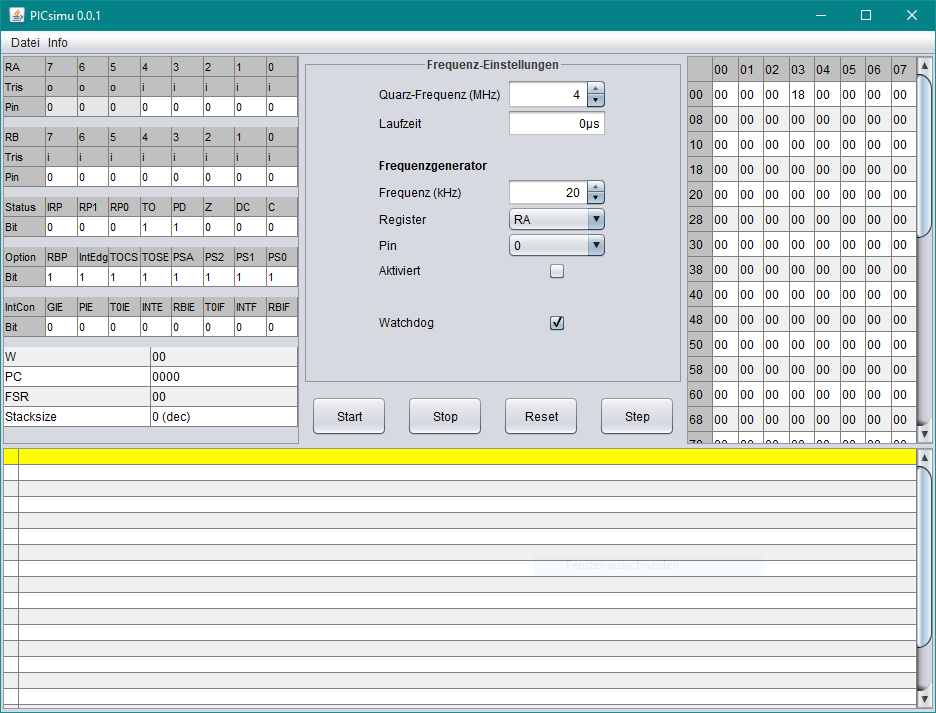
\includegraphics[width=0.8\textwidth]{img/gui}
	\caption{Die Oberfläche der Anwendung}
	\label{gui}
\end{figure}
Bei Anwendung des Dark-Modes über die Menüleiste bekommen alle Felder einen dunklen Hintergrund und eine weiße Schriftfarbe. Je nach Vorliebe kann der Benutzer sich seine präferierte Darstellung auswählen. Die grafische Oberfläche ist außerdem 'full-responsive', d.h. das Fenster kann beliebig vergrößert, und durch eingefügte Scrollbalken auch verkleinert werden, ohne dass die Oberfläche leere oder überlappende Bereiche enthält oder an Funktionialität verliert. 
Einige Einstellungsmöglichkeiten wurden zusätzlich mit Hover-Tooltip-Texten versehen, sodass auch zu lange Code-Kommentare, die Speicher-Adressen und die Laufzeit pro Befehl dargestellt werden können. 
\begin{figure}[ht]
	\centering
	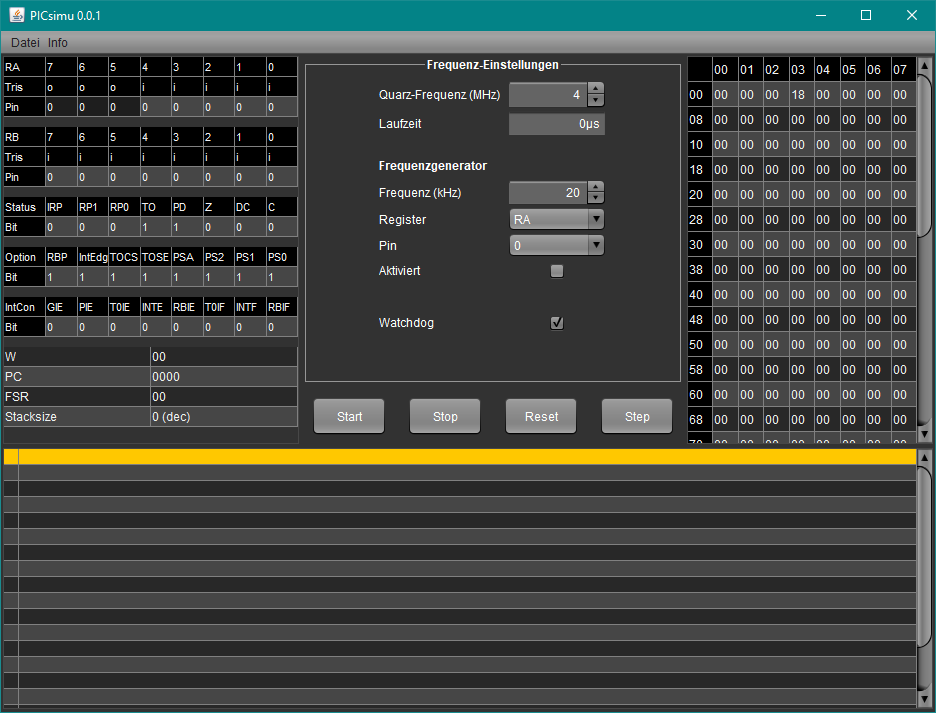
\includegraphics[width=0.8\textwidth]{img/gui-dark}
	\caption{Die Oberfläche im Dark-Mode}
	\label{gui-dark}
\end{figure}
\section{Funktionsweise}
Jeder oben genannte Bereich besteht aus mindestens einer Klasse. Für die Tabellen, die in den Registern auf der linken Seite, der Speicherdarstellung, und in der Code-Anzeige zum Einsatz kamen, wurden 'JTables' der Java-Swing Bibliothek verwendet. Das gesamte Layout beruht auf dem GridBagLayout und ist deshalb komplett responsiv. Sobald es eine Änderung in einem Bereich gibt, werden sofort alle anderen geupdatet, damit immer alles korrekt dargestellt wird. Folgende Besonderheiten gibt es zu den einzelnen Bereichen:
\begin{itemize}
	\item Die Port-Register in der linken, oberen Ecke lassen sich nur verändern, wenn die Tris-Register auf Eingang, d.h. auf 1 eingestellt sind.
	\item Die Speichertabelle auf der rechten Seite zeigt über ein Hover-Event die jeweilige Adresse als Tooltip an. Somit kann eine Adresse leichter gefunden werden. 
	\item Für die Code-Anzeige gibt es ebenfalls Tooltips der einzelnen Zeilen, in welchen mögliche Kommentare dargestellt sind. Dadurch lassen sich auch zu lange Kommentare, die über den Fensterrand hinausgehen würden, lesen. 
\end{itemize}



% Kapitel 2: Logik
\chapter{Logik}

\section{Projektstruktur}

Das Projekt lässt sich in mehrere Teilmodule (Packages) aufgliedern. Gemäß dem objektorientieren Programmieren werden Klassen, die einen logischen Zusammenhang besitzen, in ein Package zusammengefasst.

\begin{figure}[!ht]
\centering
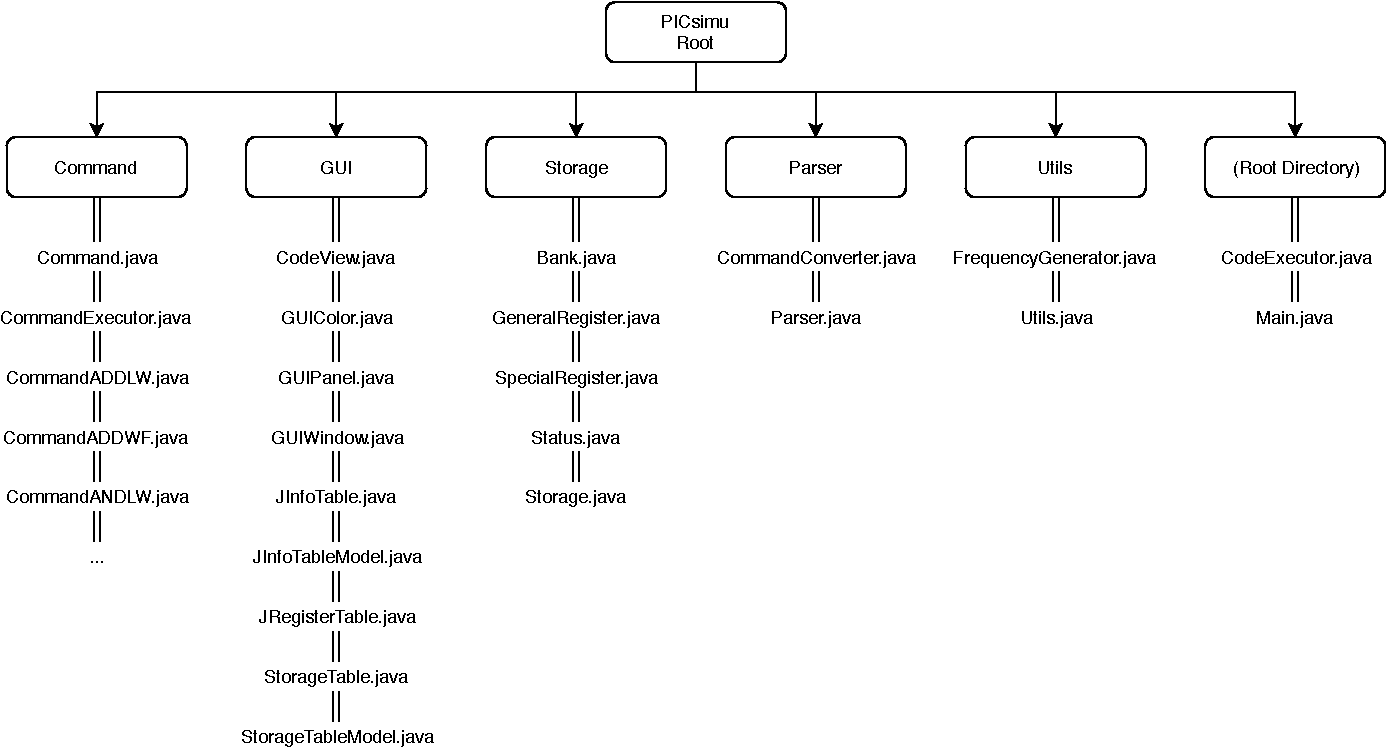
\includegraphics[width=\textwidth]{img/PICsimu-tree.pdf}
\caption{Projektstruktur-Baum}
\label{project-tree}
\end{figure}

\noindent In diesem Projekt gibt es nachfolgende Packages; es werden die darin wichtigsten Klassen erklärt.

\begin{description}
\item[Command]{Dieses Package beinhaltet die Klassen zu sämtlichen Assemblerbefehlen - von \textit{ADDLW} bis \textit{XORWF}. Zudem gibt es die Superklasse \textit{CommandExecutor} mit Methoden, welche das Status-Register nach einer Rechenoperation beeinflussen. In der Enumeration \textit{Command} werden alle Befehle aufgelistet - inklusive Befehlscode, Argumentmaske, Anzahl Quarztakte sowie die \enquote{Status Affected Bits}.}
\item[GUI]{Dieses Package beinhaltet die Klassen zur grafischen Oberfläche - dem Frontend. \textbf{TO BE CONTINUED...}}
\item[Storage]{Dieses Package beinhaltet die Klassen zum (Register-) Speicher sowie zur Bankumschaltung. Die Enumeration \textit{SpecialRegister} beinhaltet eine Auflistung der Spezialregister (z.B. Status-Register) mit deren Speicheradressen und Standardbelegung. In der Klasse \textit{Storage} wird der Speicher (inklusive EEPROM) des Mikrocontrollers verwaltet.}
\item[Parser]{Dieses Package beinhaltet die Klasses zum Parsing der Programme für den Mikrocontroller. \textbf{TO BE CONTINUED...}}
\item[Utils]{Dieses Package beinhaltet Klassen mit nützlichen (programminternen) Hilfsmethoden sowie einen einstellbaren Frequenzgenerator, der an die Pins von PORTA bzw. PORTB angelegt werden kann.}
\item[(Root Directory)]{Dieses Package ist das Root Verzeichnis der Packages. In diesem liegen alle anderen Packages sowie die Klasse \textit{Main} und \textit{CodeExecutor}. \textbf{TO BE CONTINUED...}}
\end{description}

% Kapitel 3: Fazit
\chapter{Fazit}

Das Projekt der Entwicklung eines PIC-Simulator hat sehr zum Verständnis von den Komponenten eines Mikrocontrollers beigetragen. Aufgrund von bisherigen Erfahrungen und Kenntnissen sowie der Plattformunabhängigkeit entschieden wir uns für die objektorientierte Programmiersprache Java.

Die Umsetzung in verschiedenen Klassen war sehr übersichtlich und strukturiert, sodass es kaum Probleme mit der Programmarchitektur gab. Die Darstellung jedes Kommandos in einer eigenen Klasse war zwar aufwendig, trug aber dazu bei, dass die Befehle übersichtlich und klar organisiert waren. Zudem wurde dadurch das objektorientierte Design konsequent umgesetzt.

Die Oberfläche mittels der Java Swing-Bibliothek ohne ein grafisches Fenstererstellungs-Tool ist ebenfalls gelungen, sodass am Ende sogar ein responsives Design mit allen nötigen Funktionen implementiert werden konnte. Alles in allem kann gesagt werden, dass sich die Sprache Java für die Entwicklung dieses Projektes gut eignet.

Der Quellcode dieses Projekts kann unter \href{https://github.com/teamwaldstadt/PICsimu/}{https://github.com/teamwaldstadt/PICsimu} eingesehen werden.


%%%%%%%%%%%%%%%%%%%%%%%%%%%%%%%%%%% Literaturverzeichnis %%%%%%%%%%%%%%%%%%%%%%%%%%%%%%%%%%%

%\newpage
%\pagestyle{empty}
%\pagenumbering{Roman} \setcounter{page}{\value{savepage}}


%\renewcommand{\bibname}{Literaturverzeichnis}
%\addcontentsline{toc}{chapter}{\bibname}
%\printbibliography
%\noindent Hier wird das Literaturverzeichnis (auch mit Titel) stehen!

%\newpage\null\thispagestyle{empty}\newpage % leere Seite



%%%%%%%%%%%%%%%%%%%%%%%%%%%%%%%%%%% Ende des Dokuments %%%%%%%%%%%%%%%%%%%%%%%%%%%%%%%%%%%

\end{document}
